
%(BEGIN_QUESTION)
% Copyright 2012, Tony R. Kuphaldt, released under the Creative Commons Attribution License (v 1.0)
% This means you may do almost anything with this work of mine, so long as you give me proper credit

A technician connects a DAQ (Data Acquisition) module to one phase of a 480 VAC three-phase electric motor in order to measure and record that motor's voltage and current simultaneously on a laptop computer.  The DAQ functions as a high-speed data recorder, allowing the computer to display and record a time-based graph of motor voltage and motor current over time.

Knowing that the phase-to-phase voltage of approximately 480 volts and the line current of approximately 25 amps will be far too great for the DAQ to directly measure, the technician uses {\it instrument transformers} (a ``PT'' potential transformer and a ``CT'' current transformer) to step these voltages and currents to more reasonable values:

$$\includegraphics[width=15.5cm]{i02035x01.eps}$$

Unfortunately, as soon as the motor is energized, the DAQ disappears in a bright flash of light and cloud of smoke.  The destruction also propagated to the PC the DAQ was connected to (through the USB cable)!  What went wrong, and how should the technician correct his mistake?  Assume we must use the same instrument transformers shown here, but somehow make them work with another DAQ unit having the same $\pm$ 10 volt input limits.

\vskip 20pt \vbox{\hrule \hbox{\strut \vrule{} {\bf Suggestions for Socratic discussion} \vrule} \hrule}

\begin{itemize}
\item{} What exactly does an {\it instrument transformer} do?
\item{} Could this system be made to work with a differential-input DAQ?  Why or why not?
\end{itemize}

\underbar{file i02035}
%(END_QUESTION)





%(BEGIN_ANSWER)

There are problems with {\it both} the PT circuit and the CT circuit, although the more severe of the two by far is the CT circuit.

\vskip 10pt

Hint: from the DAQ's perspective, the PT acts as an AC {\it voltage source} while the CT acts as an AC {\it current source}.  The DAQ itself acts like a voltmeter, having an extremely high input impedance (in the millions of ohms).


%(END_ANSWER)





%(BEGIN_NOTES)

The PT ratio does not step the 480 VAC down enough.  A 50:1 ratio will step 480 volts RMS down to 9.6 volts RMS, but remember that the DAQ must measure the {\it peak} voltage and not just the RMS value!  Here, the peak output of the PT with a ratio of 50:1 and 480 volts RMS at the primary winding will be approximately 13.58 volts peak, which exceeds the DAQ's input range of $\pm$ 10 volts.

\vskip 10pt

The more serious problem is in the CT circuit, where a current of approximately 1.25 amps is being forced through the DAQ's high input impedance of millions of ohms.  What we need is a low-value {\it shunt resistor} to drop a voltage within the DAQ's measurement range.  It would be advisable not to use the full $\pm$ 10 volt range, due to over-burdening the CT, so I would recommend a shunt resistor dropping mere millivolts (e.g. A precision 10 m$\Omega$ shunt resistor would work quite nicely).

\vskip 10pt

Here is a proposed solution to both problems:

$$\includegraphics[width=15.5cm]{i02035x02.eps}$$

%INDEX% Electronics review: current transformer (CT)
%INDEX% Electronics review: potential transformer (PT)
%INDEX% Electronics review: transformer ratios

%(END_NOTES)


